\documentclass[10pt,journal,compsoc]{IEEEtran}

\usepackage[pdftex]{graphicx}    
\usepackage{cite}
\usepackage{subcaption}
\usepackage{mathtools}
\hyphenation{op-tical net-works semi-conduc-tor}
\graphicspath{ {../images/} }


\begin{document}

\title{Robotics Software Engineer Nanodegree: Localization Project}

\author{Manuel Huertas L\'opez}

\markboth{Localization project, Robotics Nanodegree Program, Udacity}%
{}
\IEEEtitleabstractindextext{%

\begin{abstract}
This project involves to accurately localize a mobile robot insided a provided map in Gazebo and RViz simulation enviroments. The goal includes to build a robot model in Gazebo and utilize packages like AMCL and the Navigation Stack to succefully identifed the position of the robot in the world. As a final test the robot will be commaned to a specific location and the navigation stack will determinate the route to follow. As part of the work it is neccessary to explore, add, and tunning specific parameters corresponding to each package to achieve the best possible localization result.
\end{abstract}


\begin{IEEEkeywords}
Robot, Udacity, Monte Carlo Filter, Kalman Filter, Localization,ROS.
\end{IEEEkeywords}}


\maketitle
\IEEEdisplaynontitleabstractindextext
\IEEEpeerreviewmaketitle

\section{Introduction}
\label{sec:introduction}
\IEEEPARstart{M}{obile} robot localization is the process to determine where a robot is located with respect to its environment. It is one of the fundamental parts required by a robot to achieve autonomous navigation.

In its simplest form, position tracking, the initial robot pose is known and it is only necessary to correct incremental errors in the robot odometry. More challenging is the global localization problem, where the robot must determinate its initial pose by itself. Finally, in the kidnapped robot problem, the robot is tele-ported to other position without being told. The kidnapped problem can be used to teach the robot how to recover from a system fail, where the robot previous knowledge is complete lost.

Localization can be used in so many applications ranging from robots to clean the floors to robot to explore other planets.

The localization algorithms must overcome some difficulties like the errors in sensor measurement; like sensors to measure the distances in scene, and errors in the control. The algorithm used for the project use Bayesian probability to evaluate the probability of a hypothesis, where the robot is located, base on the observation of the environment.

\section{Background}
In the present work Kalman filter and Adaptative Monte Carlo have been evaluated. 

They are both base on probability distribution of the states over measurements using a Bayes filter. 

Adaptive Monte Carlo algorithm has been selected in order to solve the Localization problem. AMCL, a particle filter, has got so many advantages over other solutions: the error and noise does not need to follow a Gaussian distribution, the computational needs can be easily adapted, it is a very robust and fast algorithm.\cite{lamport1994latex}

\subsection{Kalman Filters}

Kalman filter was invented by Rudolf Kalman and it was used to solve non-linear problem of the trajectory estimation of the Apollo program. It helped to the Apollo to orbit around the moon. 

Kalman filter is an estimation algorithm used to estimate the value of a variable as the data is being collected. It can take data, from sensors, with a lot of uncertainty or noise in measurements and provides a very accurate estimate of the real value. It can do fast and without needing too much computer power. 

Kalman filter can be used for local localization problem where both the odometry and movement contains a lot of noise and uncertain. The Kalman filter is continuously iterating two steps: measurement update where measurement is used to update the robot's position, and state prediction where the information about current state is used to predict the future pose. At the beginning an initial guess is used. After a few iterations the measurement converge to the real value.

The Kalma filter assumes a Gaussian distribution of the noise an uncertain and it is only valid for linear system.

\begin{align}
P(x) = \frac{1}{{\sigma \sqrt {2\pi } }}e^{{{ - \left( {x - \mu } \right)^2 } \mathord{\left/ {\vphantom {{ - \left( {x - \mu } \right)^2 } {2\sigma ^2 }}} \right. \kern-\nulldelimiterspace} {2\sigma ^2 }}}
\end{align}

Nevertheless, a variation of the algorithm, Extended Kalman filter can be used for non-linear system. The EKF linearise the original non-linear filter dynamics around the previous estimates.

\subsection{Particle Filters}

The Monte Carlo localization is the most popular Localization algorithm in robotics. It can solve the local an global localization problems. The robot will navigate inside a known map collecting information using range sensors. MCL uses these sensor measurement to keep track of the robot pose. 

In MCL a set of particles are initially spread randomly and uniformly throughout the entire map. These virtual particles represents the hypothesis of where the robot might be. In a 2D map, each particle has got a position , orientation and weight value. The importance of a particle depends on the weight, the bigger the more accurate and during the re-sampling process they are more likely to survive. After several iterations of the Monte Carlo algorithm the particles will converge and estimate the robot's pose.

The MCL uses a Bayes filtering to estimate a probability density over the state space conditioned by the measurement, this probability density is called belief:

\begin{align}
Bel(X{t}) = P(X{t} |Z{1}...{t} )
\end{align}

X{t} are the state of robot and Z are the measurement from time 1 up to time {t}. The belief is estimated recursively, the initial guess uses a randomly and uniformly distribution over the entire map.

The MCL has got two sections. In every iteration the algorithm takes: previous belief, the actuation commands and the sensor measurement as input. The hypothetical state is computed whenever the robot moves, the particles weight are computed using the latest sensor measurement. Secondly the particles with high probability, the ones that fetch better the measurement reading, will survive and the others will die. The algorithm will output the new belief of the next iteration. After few iterations the survivors particles will represent the real robot's pose.


\subsection{Comparison / Contrast}

MCL presents many advantages over EFK:

\begin{itemize}
\item MCL is easier to program than EFK 
\item In the EFK algorithm the noise error and uncertain must follow a Gaussian distribution, MCL is not tied to the measure noise distribution.
\item MCL can control the computational memory and resolution of the solution by changing the number of particles distributed.
\end{itemize} 

In the present work MCL particle filter is going to be used.


\section{Simulations}
The simulation environment selected was Gazebo, connected to ROS a Rviz to visualize the performance of the solution. 

ROS is a meta-operating system for robotic. It provides a broad collection of libraries, in the form of packages, that implement useful robot functionality. ROS provides publish-subscribe messaging infrastructure that allows easily integrate different package to implement the particular solution.

The following sections will explain in details the robot's model, selected packages, and the parameter tunning to allow the robot to properly localize itself.

\subsection{Achievements}
Two different models have been evaluated: one provided by Udacity and other built from scratch.

The following sections include the model design for each one, the package used to create the navigation stack and the parameters selected, with its meaning, in order to obtain the desire performance.
% Robot Models
\subsection{Benchmark Model}


\subsubsection{Model design}
The Robot's design considerations should include: the size of the robot, the layout of sensors. This information can be shown in the form of a chart / table.

\begin{figure}
    \centering
    \begin{subfigure}[b]{0.3\textwidth}
        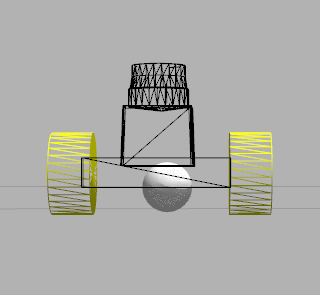
\includegraphics[width=\textwidth]{robokoko-design-1}
        \caption{A gull}
        \label{fig:gull}
    \end{subfigure}
    \begin{subfigure}[b]{0.3\textwidth}
        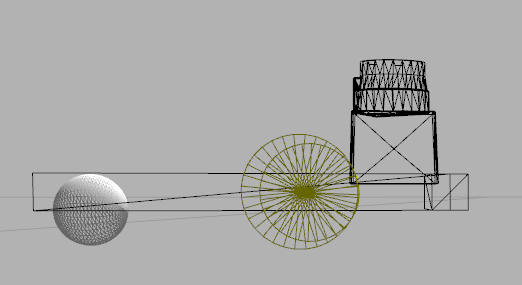
\includegraphics[width=\textwidth]{robokoko-design-2}
        \caption{A tiger}
        \label{fig:tiger}
    \end{subfigure}
    \begin{subfigure}[b]{0.3\textwidth}
        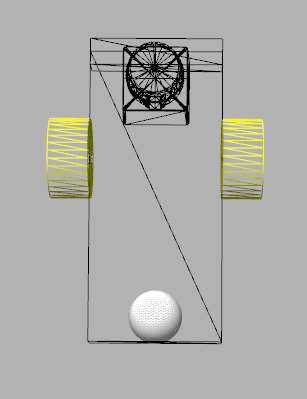
\includegraphics[width=\textwidth]{robokoko-design-3}
        \caption{A mouse}
        \label{fig:mouse}
    \end{subfigure}
    \caption{Robot desing view}\label{fig:animals}
\end{figure}


\subsubsection{Packages Used}
The packages used in the project should be specified as well as the topics received and published; the services it used and provided should also be addressed. 

\subsubsection{Parameters}
Localization parameters in the AMCL node should be described, as well as move\_base parameters in the configuration file. You should be able to clearly demonstrate your understanding of the impact of these parameters.

\subsection{Personal Model}

\subsubsection{Model design}

\begin{figure}
    \centering
    \begin{subfigure}[b]{0.3\textwidth}
        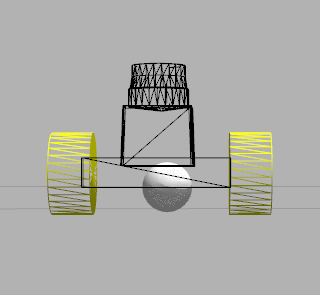
\includegraphics[width=\textwidth]{robokoko-design-1}
        \caption{A gull}
        \label{fig:gull}
    \end{subfigure}
    \begin{subfigure}[b]{0.3\textwidth}
        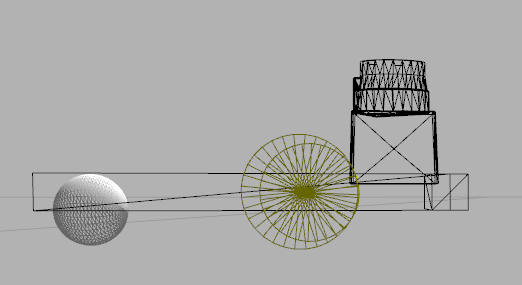
\includegraphics[width=\textwidth]{robokoko-design-2}
        \caption{A tiger}
        \label{fig:tiger}
    \end{subfigure}
    \begin{subfigure}[b]{0.3\textwidth}
        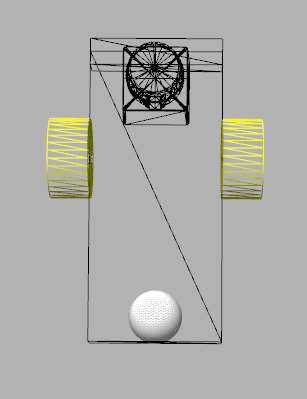
\includegraphics[width=\textwidth]{robokoko-design-3}
        \caption{A mouse}
        \label{fig:mouse}
    \end{subfigure}
    \caption{Robot desing view}\label{fig:animals}
\end{figure}

\begin{itemize}
\item Chassis:
\item Wheels:
\item Back caster:
\item Lidar:
\item Camera:
\end{itemize}

\subsubsection{Packages Used}

\begin{itemize}
\item gazebo\_ros:
\item rviz:
\item map\_server:
\item tf:
\item amcl:
\item move\_base: 
\end{itemize}

\subsubsection{Parameters}

\paragraph{Localization parameters}

The package for localization used was AMCL. There are several parameters to be tuned:

The following configuration parameters were chosen due to power limitations of the computer where packages were deployed, increasing this values may produced a better performance.

\begin{itemize}
\item min\_particles[100]: Minimum allowed number of particles spread around the scene.
\item max\_particles[5000]: Maximum allowed number of particles spread around the scene. 
\item transform\_tolerance[0.5]: It is used to make a transformation valid in the future in order to cover lag in the system. Reducing this value improve performance but it is necessary to have computer power enough.
\item gui\_publish\_rate[1]: Maximum rate (Hz) at which scans and paths are published for visualization.
\end{itemize}

Parameters related to how recovering from stuck:

\begin{itemize}
\item recovery\_alpha\_slow[0.001]: Exponential decay rate for the slow average weight filter, used in deciding when to recover by adding random poses.   
\item recovery\_alpha\_fast[0.1]: Exponential decay rate for the fast average weight filter, 
used in deciding when to recover by adding random poses.
\end{itemize}

The following parameters give and estimation of the initial pose, mean and covariance, of the robot in the world, previous to any movement:

\begin{itemize}
\item initial\_pose\_x[0.0]: Initial pose mean (x), used to initialize filter with Gaussian distribution.
\item initial\_pose\_y[0.0]: Initial pose mean (y), used to initialize filter with Gaussian distribution.
\item initial\_pose\_a[0.0]: Initial pose mean (yaw), used to initialize filter with Gaussian distribution.
\item initial\_cov\_xx[0.25]: Initial pose covariance (x*x), used to initialize filter with Gaussian distribution.
\item initial\_cov\_yy[0.25]: Initial pose covariance (y*y), used to initialize filter with Gaussian distribution.
\item initial\_cov\_aa[0.07]: Initial pose covariance (yaw*yaw), used to initialize filter with Gaussian distribution.
\end{itemize}

Parameters related to the Laser and model configuration:

\begin{itemize}
\item laser\_likelihood\_max\_dist[2.0]: Maximum distance to do obstacle inflation on map, for use in likelihood\_field model.
\item laser\_model\_type[likelihood\_field]: Which model to use, either beam, likelihood\_field.
\item odom\_model\_type[diff\-corrected]: Which model to use, either "diff", "omni", "diff-corrected" or "omni-corrected". In our case the robot is diff type, the corrected include a bug correction.
\end{itemize}

The following parameters are about the noise in odemotry measurement. Because we are using a Bayesian Filter the probability of true values of odometry can be tuned using these parameters. These values where obtained by trail and error.

\begin{itemize}
\item odom\_alpha1[0.005]: Specifies the expected noise in odometry's rotation estimate from the rotational component of the robot's motion.
\item odom\_alpha2[0.005]: Specifies the expected noise in odometry's rotation estimate from translational component of the robot's motion. 
\item odom\_alpha3[0.010]: Specifies the expected noise in odometry's translation estimate from the translational component of the robot's motion. 
\item odom\_alpha4[0.010]: Specifies the expected noise in odometry's translation estimate from the rotational component of the robot's motion.
\end{itemize}

\paragraph{Move base parameters}

The navigation stack uses cost-maps to store information about the obstacles in the world.


Costmap common parameters:

\begin{itemize}
\item obstacle\_range[2.5]: The robot will only update its map with information about obstacles that are within 2.5 meters of the base.
\item raytrace\_range[3.0]: This parameter determines the range to which we will raytrace freespace given a sensor reading. The robot will attempt to clear out space in front of it up to 3.0 meters away given a sensor reading.
\item robot\_radius[0.11]: The robot radius is 11cm. It's used to avoid passing the robot through narrow places where it can get stuck.
\item inflation\_radius[0.2]: The robot will treat all paths that stay 0.2 meters or more away from obstacles as having equal obstacle cost.
\end{itemize}

The local costmap is used by the local planner to generate a short-term plan. The local costmap uses the odometry information rather than a map.

\begin{itemize}
\item robot\_base\_frame: 
\item update\_frequency[2]: The frequency, in Hz, at which the cost-map will run its update loop. 
\item publish\_frequency[2]: The rate, in Hz, at which the cost-map will publish visualization information.
\item width[20.0]: The cost-map's width.
\item height[20.0]: The cost-map's height.
\item resolution[0.05]: The cost-map's resolution.
\item static\_map[false]: The costmap should not initialize itself based on a map served by the map\_server, for the local costmap the odometry is used.
\item rolling\_window[true]:  the robot only cares about obstacles within a local area.
\item transform\_tolerance[0.5]: Specifies the delay in transform (tf) data that is tolerable in seconds.
\end{itemize}

The global costmap is used by the local planner to generate a long-term plan. The global costmap uses the map provided by the map\_server.

\begin{itemize}
\item robot\_base\_frame:
\item update\_frequency[2]: The frequency, in Hz, at which the cost-map will run its update loop. 
\item publish\_frequency[2]: The rate, in Hz, at which the cost-map will publish visualization information.
\item width[40.0]: The cost-map's width.
\item height[40.0]:The cost-map's height.
\item resolution[0.05]: The cost-map's resolution.
\item static\_map[true]: The costmap should initialize itself based on a map served by the map\_server.
\item rolling\_window[false]: for global localization this parameter must set to false.
\item transform\_tolerance[0.5]: Specifies the delay in transform (tf) data that is tolerable in seconds. 
\end{itemize}

This package provides implementations of the Trajectory Rollout and Dynamic Window approaches to local robot navigation on a plane. Given a plan to follow and a costmap, the controller produces velocity commands to send to the robot.

\begin{itemize}
\item holonomic\_robot[false]: Determines whether velocity commands are generated for a holonomic or non-holonomic robot. Our model is not holonomic.
\item sim\_time[2.0]: The amount of time to forward-simulate trajectories in seconds. This values was selected due to computer power restrictions.
\item meter\_scoring[true]: Whether the gdist\_scale and pdist\_scale parameters should assume that goal\_distance and path\_distance are expressed in units of meters or cells.
\item max\_vel\_x[0.4]: The maximum forward velocity allowed for the base in meters/sec.
\item min\_vel\_x[0.1]: The minimum forward velocity allowed for the base in meters/sec.
\item max\_vel\_theta[0.7]: The maximum rotational velocity allowed for the base in radians/sec.
\item min\_vel\_theta[-0.7]: The minimum rotational velocity allowed for the base in radians/sec.
\item acc\_lim\_x[0.6]: The x acceleration limit of the robot in meters/sec\^2.
\item acc\_lim\_y[0.6]: The y acceleration limit of the robot in meters/sec\^2.
\item acc\_lim\_theta[1.5]: The rotational acceleration limit of the robot in radians/sec\^2.
\end{itemize}

\section{Results}
Present an unbiased view of your robot's performance and justify your stance with facts. Do the localization results look reasonable? What is the duration for the particle filters to converge? How long does it take for the robot to reach the goal? Does it follow a smooth path to the goal? Does it have unexpected behavior in the process? \\
For demonstrating your results, it is incredibly useful to have some watermarked charts, tables, and/or graphs for the reader to review. This makes ingesting the information quicker and easier.

\subsection{Localization Results}
\subsubsection{Benchmark}
\subsubsection{Student}

\subsection{Technical Comparison} % only facts
Discuss the difference of the layout, parameters, performance etc. between the benchmark robot and your robot. It is acceptable for your custom robot to perform worse than the provided robot. The focus is on learning and understanding, not performance. 

\section{Discussion}
This is the only section of the report where you may include your opinion. However, make sure your opinion is based on facts. If your robot performed poorly, make mention of what may be the underlying issues. If the robot runs well, which aspects contribute to that? Again, avoid writing in the first person (i.e. Do not use words like "I" or "me"). If you really find yourself struggling to avoid the word "I" or "me"; sometimes, this can be avoid with the use of the word “one”. As an example: instead of : "I think the robot cannot localize itself because the sensor does not provide enough information for localization" try: "one may believe the localization performance is poor because the sensor layout is not able to provide enough information for localization". They say the same thing, but the second avoids the first person. 

\subsection{Topics}

\begin{itemize}
\item Which robot performed better?
\item Why it performed better? (opinion)
\item How would you approach the 'Kidnapped Robot' problem?
\item What types of scenario could localization be performed?
\item Where would you use MCL/AMCL in an industry domain?
\end{itemize}

\section{Conclusion / Future work}
This section is intended to summarize your report. Your summary should include a recap of the results, did this project achieve what you attempted, how would you deploy it on hardware and how could this project be applied to commercial products? 
For Future Work, address areas of work that you may not have addressed in your report as possible next steps. This could be due to time constraints, lack of currently developed methods / technology, and areas of application outside of your current implementation. Again, avoid the use of the first-person.

\subsection{Modifications for Improvement}
Examples:

\begin{itemize}
\item Base Dimension
\item Sensor Location
\item Sensor Layout
\item Sensor Amount
\end{itemize}

\subsection{Hardware Deployment}

\begin{enumerate}
\item What would need to be done?
\item Computation time/resource considerations?
\end{enumerate}



\bibliography{bib}
\bibliographystyle{ieeetr}

\end{document}